\subsection{Importanza e motivazioni dell’Ingegneria del SW (IS)}
\begin{itemize}
    \item Le economie di TUTTE le nazioni sviluppate dipendono da software
    \item Sempre più sistemi sono controllati da software
    \item \textbf{\underline{L'ingegneria del software si occupa}} di teorie, metodi e strumenti per lo sviluppo di software professionale
    \item Le spese di ingegneria del software rappresentano una frazione significativa del PNL (Prodotto nazionale lordo) in tutti i paesi sviluppati
\end{itemize}

\subsection{L’aspetto economico: i costi del SW: manutenzione vs. sviluppo; costruzione vs. testing; distribuzione dei costi dei vari processi sw}
\begin{itemize}
    \item Di solito il software costa più del hardware
    \item I costi di manutenzione di un software possono essere più elevati (anche diverse volte) dei costi di sviluppo
    \item L'ingegneria del software si occupa dello sviluppo di software economico (ciclo di vita del software quindi sviluppo e manutenzione)
\end{itemize}

\subsection{SW include documentazione}
\begin{itemize}
    \item Il software è il programma \textbf{\underline{e}} la documentazione
\end{itemize}

\subsection{SW generico vs. SW customizzato, sw re-use}
\begin{itemize}
    \item Generico: sviluppato per essere venduto a diversi clienti (Microsoft office, Antivirus, programmi CAD, anche software per un market specifico sono generici (dentisti))
    \item Customizzato (personalizzato/personalizzato): sviluppato per un singolo cliente in base alle loro specifiche/esigenze
    \item Un software può essere sviluppato in tre modi:
    \begin{enumerate}
        \item Da zero
        \item Customizzando un software generico
        \item Riutilizzando un software esistente
    \end{enumerate}
    \item Le specifiche del software appartengono a enti diverse in base al tipo di software (generico/customizzato)
    \begin{itemize}
        \item nel primo caso appartengono a chi lo sviluppa e le decisioni per le modifiche del software possono essere fatte dagli sviluppatori
        \item nel secondo caso appartengono al cliente e le decisioni per le modifiche del software sono richieste dal cliente
    \end{itemize}
\end{itemize}

\subsection{Definizioni e limiti di IS; system engineering}
\begin{itemize}
    \item L'ingegneria dei sistemi si occupa di tutti gli aspetti dello sviluppo di sistemi basati su computer, inclusi hardware, software e ingegneria dei processi
    \item L'ingegneria dei sistemi è parte del processo
    \item I System engineers sono coinvolti nelle specifiche di sistema, nella progettazione dell'architettura, nell'integrazione e nella distribuzione
\end{itemize}

\subsection{Prime definizioni di alcuni processi fondamentali (spec, design, development, programming, integration, validation, deploy, evolution)}
\begin{itemize}
    \item Requirement Analysis: dove le esigenze dei clienti vengono acquisite, scoperte e analizzate dai tecnici del software
    \item Specification: in cui i clienti e gli ingegneri del software definiscono il software che deve essere prodotto e i vincoli sul suo funzionamento
    \item Development: produzione (progettazione e programmazione/progettazione e realizzazione) del sistema software
    \item Validation: verifica che il software sia ciò che il cliente richiede
    \item Evolution: modifica del software per riflettere le mutevoli esigenze dei clienti e del mercato
\end{itemize}

\subsection{Ragionamento ANALITICO e R. SINTETICO}
\begin{itemize}
    \item Analitico: Dato un problema analizzo le parti del problema e risolvo le parti una alla volta ciò permette di andare nel dettaglio
    
    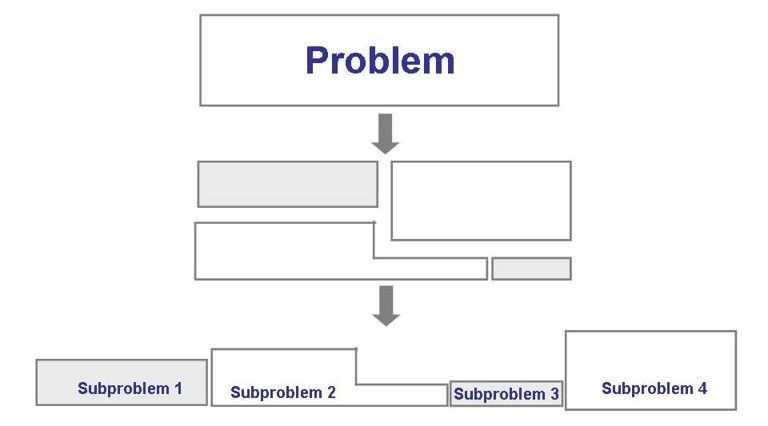
\includegraphics[width=\textwidth]{analysis}
    \item Sintetico: Costruisco dai sotto-problemi la soluzione al problema di partenza
    
    L'integrazione dei sotto-problemi è difficile
    
    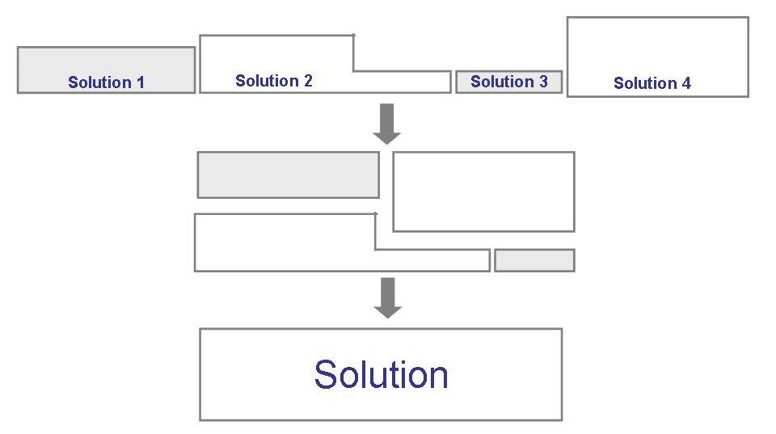
\includegraphics[width=\textwidth]{synthesis.jpg}
\end{itemize}

\subsection{Processo SW; MODELLO dei Processi SW; modelli generici}
\begin{itemize}
    \item Processo Software: Un insieme di attività correlate il cui obiettivo è lo sviluppo o l'evoluzione del software
    \item Modello dei processi: Una rappresentazione semplificata di un processo software, presentata da una prospettiva specifica
    \item Modelli generici: Waterfall, Evolutionary development, Formal transformation, Integration from reusable components, \dots 
\end{itemize}

\subsection{Parametri di Qualità del SW: manutenibilità, ‘potersi fidare’, sicurezza \& protezione, efficienza, accettabilità}
\begin{itemize}
    \item Manutenibilità: Il software deve poter evolversi facilmente per soddisfare le mutevoli esigenze
    \item Affidabilità e sicurezza: Il software deve essere affidabile, sicuro (Protezione: non danneggiare i propri dati) e protetto (Sicurezza: non provocare danni a cose, persone, \dots)
    \item Efficienza: Il software non dovrebbe fare uno spreco di risorse di sistema (non è più un problema così importante come in passato)
    \item Accettabilità: Il software deve essere accettabile per il tipo di utenti per cui è progettato. Ciò significa che deve essere comprensibile, utilizzabile e compatibile con altri sistemi che usano
\end{itemize}

\subsection{Le grandi sfide attuali dell’IS: sistemi Legacy, eterogeneità hd e SW, richiesta di velocità nello sviluppo e nella delivery}
\begin{itemize}
    \item Legacy system: sistemi vecchi e preziosi devono essere mantenuti e aggiornati
    \item Eterogeneità: sempre più spesso i sistemi devono funzionare come sistemi distribuiti su reti che includono diversi tipi di computer e dispositivi mobili
    \item Consegna, sicurezza e fiducia: i cambiamenti aziendali, sociali e culturali stanno causando una crescente pressione per una consegna più rapida del software
\end{itemize}

\subsection{Web e IS}
\begin{itemize}
    \item Il Web è ora una piattaforma per l'esecuzione di applicazioni e organizzazioni stanno sviluppando sempre più sistemi basati sul Web piuttosto che sistemi locali.
    \item I servizi Web consentono l'accesso alle funzionalità dell'applicazione sul Web.
    \item Il cloud computing è un approccio alla fornitura di servizi informatici in cui le applicazioni vengono eseguite in remoto sul "cloud".
    \item Gli utenti non acquistano software ma pagano in base all'uso (SaS - Software ad a Service).
    \item Il riutilizzo del software è l'approccio dominante per la costruzione di sistemi basati sul Web.
    \item I sistemi basati sul Web dovrebbero essere sviluppati e distribuiti in modo incrementale.
    \item Le interfacce utente sono vincolate dalle capacità dei browser Web.
\end{itemize}